\documentclass[a4paper,11pt]{article}
\title{Investigation of Damped Oscillators}
\author{Izaak van Dongen}

% make the document take up more of the page
\usepackage[margin=1in,headheight=13.6pt]{geometry}

% so the title can be accessed by fancyhdr (and is automatically correctly
% spelled etc)
\makeatletter
\let\thetitle\@title
\makeatother

% custom document header/footer
\usepackage{fancyhdr}
\usepackage{lastpage}

\pagestyle{fancy}
\fancyhf{}
\lhead{\thetitle}
\rhead{Izaak van Dongen}
\rfoot{Page \thepage\ of \pageref{LastPage}}

%% fonts
%\usepackage[p,osf]{cochineal}
%\usepackage[scale=.95,type1]{cabin}
%\usepackage[cochineal,bigdelims,cmintegrals,vvarbb]{newtxmath}
%% fixed width font with 80 chars per listing line
%\usepackage[scaled=.94]{newtxtt}
%\usepackage[cal=boondoxo]{mathalfa}
\usepackage{amsfonts}

% provides eg uptau
\usepackage{upgreek}

% maths symbols and other stuff (supersedes the ams* packages)
\usepackage{mathtools}

% for typesetting differentials
\usepackage{commath}

% no paragraph indent
\usepackage[parfill]{parskip}

% pretty table rules and multirow entries. Also page-breaking tables
\usepackage{booktabs}
\usepackage{multirow}
\usepackage{longtable}

% plotting mathematical functions (needs version request)
\usepackage{pgfplots}
\pgfplotsset{compat=1.15}

% \url function and clickable table of contents. no ugly red boxes though
\usepackage[hidelinks]{hyperref}

% For framing definitions
\usepackage[framemethod=tikz]{mdframed}
\usepackage[most]{tcolorbox}

\newtcolorbox{definition}{
freelance,
before=\par\vspace{2\bigskipamount}\noindent,
after=\par\bigskip,
frame code={
  \node[
  anchor=south west,
  inner xsep=8pt,
  xshift=8pt,
  rounded corners=5pt,
  font=\bfseries\color{white},
  fill=gray] at (frame.north west) (tit) {\strut Definition:};
  \draw[
  line width=3pt,
  rounded corners=5pt,gray
  ] (tit.west) -| (frame.south west) -- ([xshift=15pt]frame.south west);
},
interior code={},
top=2pt
}

% for better table of contents stuff, providing the \listof* commands and not
% listing the tables in the table of contents
\usepackage[nottoc,notlof,notlot]{tocbibind}

% more advanced handling of utf8 and fonts or something. apparently good to have
\usepackage[utf8]{inputenc}
\usepackage[T1]{fontenc}

% somehow this fixes ~ signs in listing environments
\usepackage{lmodern}

% bibliography management with square braces for citations
\usepackage[square,numbers]{natbib}

% graphics, like eps files and stuff (supersedes graphics)
\usepackage{graphicx}

% used to horizontally align floats
\usepackage{subfig}

% used for figures
\usepackage{float}

% needed for colouring and stuff (xcolor supersedes color)
\usepackage{xcolor}

\definecolor{codegreen}{rgb}{ 0,0.6,0}

% listings of code
\usepackage{minted}
\setminted{breaklines,
           breakbytokenanywhere,
           linenos
}
\usemintedstyle{friendly}
% bigger line numbers
\renewcommand\theFancyVerbLine{\footnotesize\arabic{FancyVerbLine}}

% that can break across pages while being captioned figures
\usepackage{caption}
\newenvironment{longlisting}
{\addvspace{\baselineskip}\captionsetup{type=listing}}
{\addvspace{\baselineskip}}

% allow maths to break across pages
\allowdisplaybreaks

\usepackage[separate-uncertainty]{siunitx}

\begin{document}
    \maketitle%\thispagestyle{empty} % no page number under title

\begin{longlisting}
\inputminted{R}{analyse.r}
\caption{Source code of the program \texttt{analyse.r}.}
\label{lst:analyse}
\end{longlisting}

\begin{longlisting}
\inputminted{text}{analysis_output.txt}
\caption{Output of \texttt{analyse.r} (\ref{lst:analyse}) when run.}
\label{lst:results}
\end{longlisting}

\begin{figure}[H]
\begin{center}
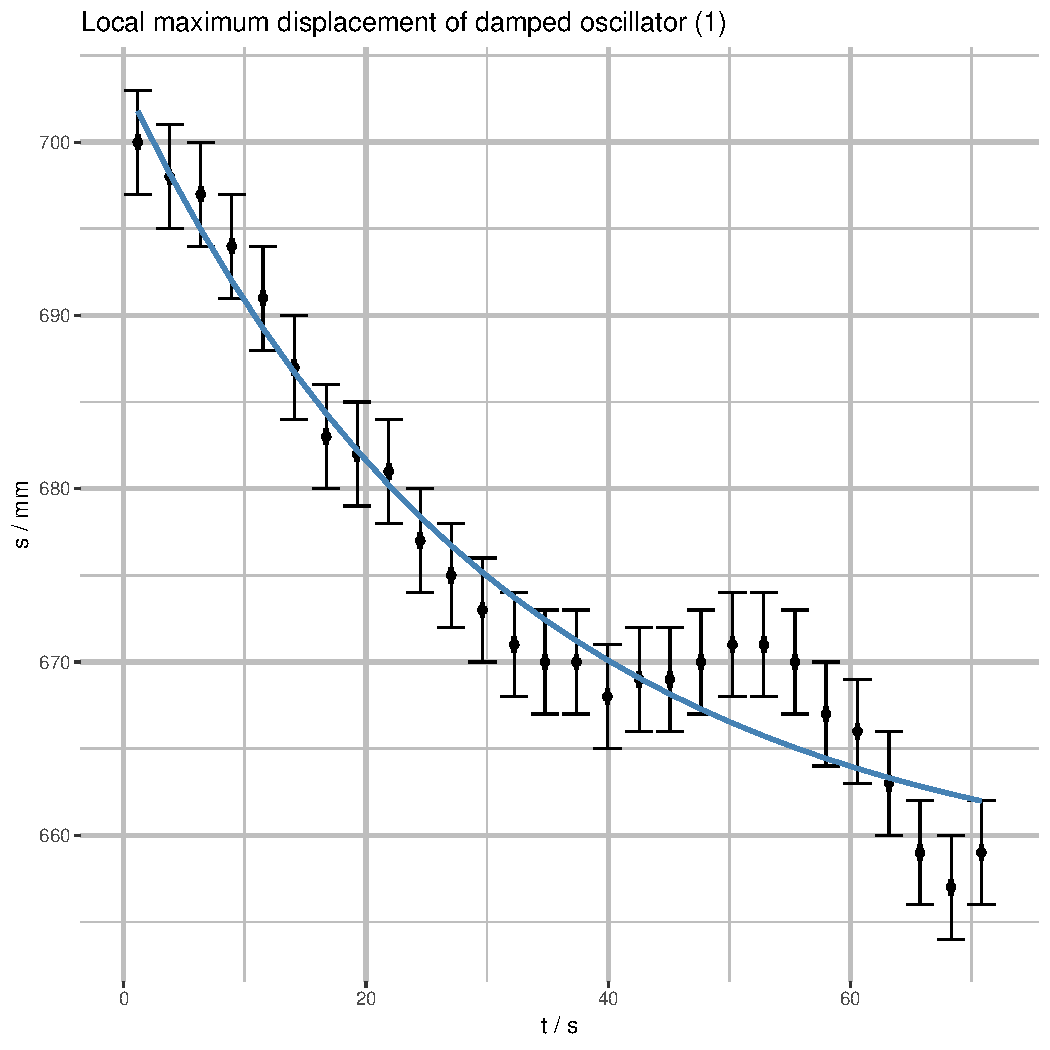
\includegraphics[height=0.45\textheight,page=1]{Rplots.pdf}
\end{center}
\caption{Plot of maximum displacements in experiment 1.}
\label{fig:ex1}
\end{figure}

\begin{figure}[H]
\begin{center}
\includegraphics[height=0.45\textheight,page=2]{Rplots.pdf}
\end{center}
\caption{Plot of maximum displacements in experiment 2.}
\label{fig:ex2}
\end{figure}

\begin{figure}[H]
\begin{center}
\includegraphics[height=0.45\textheight,page=3]{Rplots.pdf}
\end{center}
\caption{Plot of maximum displacements in experiment 3.}
\label{fig:ex3}
\end{figure}

\begin{figure}[H]
\begin{center}
\includegraphics[height=0.45\textheight,page=4]{Rplots.pdf}
\end{center}
\caption{Plot of maximum displacements in experiment 4.}
\label{fig:ex4}
\end{figure}

We did four experiments, filming each, and then used the video to find the time
and value of displacement at each local point of maximum displacement. In a
damped system,
\\$s  = Ae^{-\frac t\uptau} \cos \omega t$, so by plotting the maxima we should
get a plot of $s = Ae^{-\frac t\uptau}$. However this formula is somewhat
oversimplified as it assumes the first peak is when $t = \SI{0}{\second}$, and
that $s$ is measured from the equilibrium point. Therefore, the fully qualified
model is
\\$s = s_0 + Ae^{-\frac {t-t_0}\uptau}$.

We did directly measure values for $s_0$, but there would be considerable
uncertainties in these as the whole system was somewhat volatile and hard to
measure. Because of this uncertainty, $A$ is in a similar boat. $t_0$, on the
other hand, we know with (un)certainty, as this is simply the first $t$ value we
decide to plot.

In view of these observations, I decided to use the measurements for $s_0$
merely as starting values for the model, but to set $t_0$ as a known constant,
in the model in Listing \ref{lst:analyse}. This model was used to find $\uptau$.

I also worked out the period of oscillation $T$ for each experiment by finding
the gradient of $t_n$ with respect to $n$, where $t_n$ is the time of the $n$th
observed peak. I took this approach as this would minimise the uncertainty in
the final answer, and graphical presentation of each set of $t$ values would be
challenging, enjoyable, and allow an inspection of whether or not, for example,
$T$ is variable.

Fortunately, as you can see in Figure \ref{fig:period}, this approach produces
some very straight lines with mildly differing gradients.

\begin{figure}[H]
\begin{center}
\includegraphics[width=0.9\textwidth,page=5]{Rplots.pdf}
\end{center}
\caption{Plot of $t_n/\si{\second}$, the time of the $n$th peak, against $n$.}
\label{fig:period}
\end{figure}

From these two results, $t$ and $\uptau$, I can now calculate the $Q$-factor as
$\displaystyle Q = \frac {\pi\uptau} T$. The results are shown in Listing
\ref{lst:results}, but are presented below for your convenience, together with
the diameter of the damper used.

\begin{center}
\begin{tabular}{c S[table-format=3.0]
                  S[table-format=1.2,round-mode=places,round-precision=2]
                  S[table-format=1.2,round-mode=places,round-precision=2]
                  S[table-format=1.2,round-mode=places,round-precision=2]}
\toprule
\bfseries Experiment & {\boldmath $d / \si{\milli\metre}$} &
                       {\boldmath $\uptau / \si{\second}$} &
                       {\boldmath $T / \si{\second}$} &
                       {\boldmath $Q$} \\
\midrule
1 & 300 & 31.42320 & 2.581346 & 38.2431831229393 \\
2 & 340 & 19.05933 & 2.6146520 & 22.9004293181007 \\
3 & 405 & 17.66282 & 2.654921 & 20.9005766245794 \\
4 & 450 & 6.095009 & 2.720947 & 7.0372680956032 \\
\bottomrule
\end{tabular}
\end{center}

This would suggest that $Q$, and $\uptau$ all decrease when the area of the
damper increases, while $T$ also increases. This makes sense, and fits with the
theory I know.

In evaluation, the biggest problem we had was an interfering oscillation from
the damping card, which rotated about the point at which it was fixed to the
mass. This resulted in a sinusoidy shape being added to some of our decay
graphs, which made analysis of our data a bit trickier. The way to fix this
would probably be to devise some way to more rigidly attach the damper to the
mass. This problem was possible to work around with some of the data, but
somewhat jeopardised other parts.

\end{document}
